\section{Results}
\subsection{Initial results}
\begin{figure}
	\centering
	\begin{subfigure}[b]{0.24\linewidth}
		\centering
		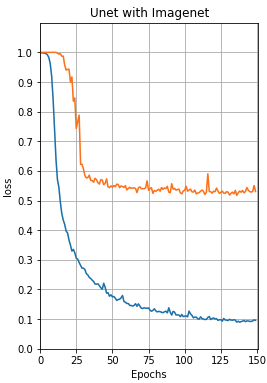
\includegraphics[width=\linewidth]{Materials/Results/Initial/UnetImagenet}
		\caption{U-Net model whose weights are initialized with ImageNet weights.}
	\end{subfigure}
	\hfill
	\begin{subfigure}[b]{0.24\linewidth}
		\centering
		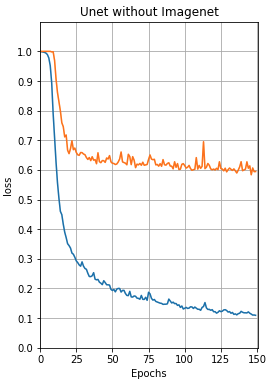
\includegraphics[width=\linewidth]{Materials/Results/Initial/UnetNoImagenet}
		\caption{U-Net model whose weights are not initialized with ImageNet weights.}
	\end{subfigure}
	\hfill
	\begin{subfigure}[b]{0.24\linewidth}
		\centering
		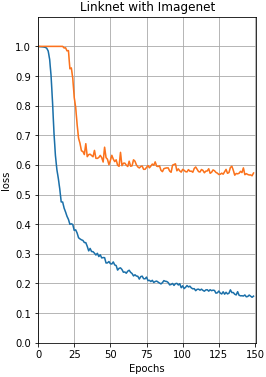
\includegraphics[width=\linewidth]{Materials/Results/Initial/LinknetImagenet}
		\caption{LinkNet model whose weights are initialized with ImageNet weights.}
	\end{subfigure}
	\hfill
	\begin{subfigure}[b]{0.24\linewidth}
		\centering
		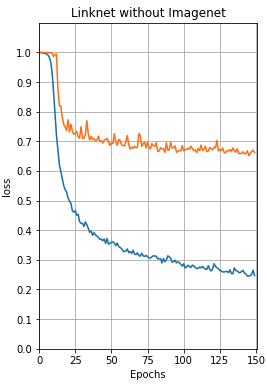
\includegraphics[width=\linewidth]{Materials/Results/Initial/LinknetNoImagenet}
		\caption{LinkNet model whose weights are not initialized with ImageNet weights.}
	\end{subfigure}
	\caption{All models are trained on the original and halved training data. The blue graphs indicates training loss measured with DICE, and the orange graphs indicates validation loss also measured with DICE.}
	\label{imagenet}
\end{figure}
Early in the project the models described in \autoref{models} were trained on the original training set. In \autoref{imagenet} we see the training and validation loss measured in DICE for each of the models. We see that all models could probably still achieve lower training loss, but after 150 epochs both U-Net models achieve lower training loss than the LinkNet model using Imagenet weights, and a lot lower training loss than the LinkNet model not using ImageNet weights. Looking at the validation loss, the two models using ImageNet weights shows the lowest loss with the U-Net model using ImageNet weights having slightly lower loss than the LinkNet model using ImageNet weights.

\begin{figure}[H]
	\centering
	\begin{subfigure}[b]{0.19\linewidth}
		\centering
		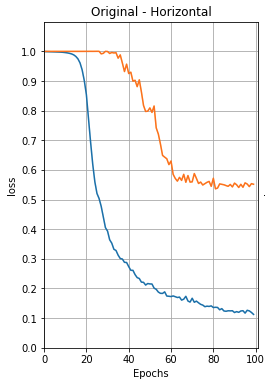
\includegraphics[width=\linewidth]{Materials/Results/Augmentation/OH}
		\caption{Original and horizontal data model.\\}
	\end{subfigure}
	\hfill
	\begin{subfigure}[b]{0.19\linewidth}
		\centering
		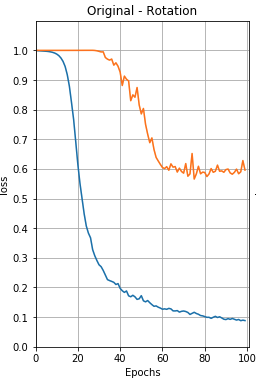
\includegraphics[width=\linewidth]{Materials/Results/Augmentation/OR}
		\caption{Original and large rotations model.\\}
	\end{subfigure}
	\hfill
	\begin{subfigure}[b]{0.19\linewidth}
		\centering
		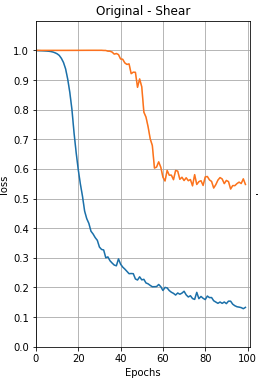
\includegraphics[width=\linewidth]{Materials/Results/Augmentation/OS}
		\caption{Original and large shearing model.\\}
	\end{subfigure}
	\hfill
	\begin{subfigure}[b]{0.19\linewidth}
		\centering
		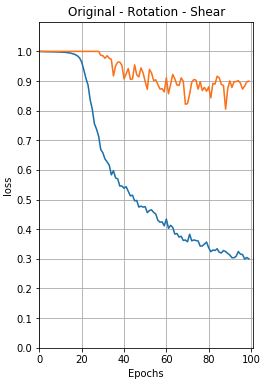
\includegraphics[width=\linewidth]{Materials/Results/Augmentation/ORS}
		\caption{Original, large rotation and large shearing model.}
	\end{subfigure}
	\hfill
	\begin{subfigure}[b]{0.19\linewidth}
		\centering
		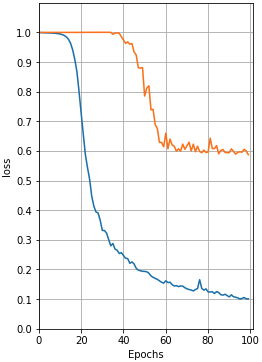
\includegraphics[width=\linewidth]{Materials/Results/Augmentation/ORHV}
		\caption{Original, large rotation, horizontal and vertical model.}
	\end{subfigure}
	\\
	\begin{subfigure}[b]{0.19\linewidth}
		\centering
		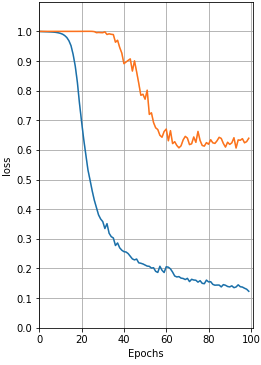
\includegraphics[width=\linewidth]{Materials/Results/Augmentation/ORHVS}
		\caption{Original, large rotation, large shearing, horizontal and vertical model.}
	\end{subfigure}
	\hfill
	\begin{subfigure}[b]{0.19\linewidth}
		\centering
		\includegraphics[width=\linewidth]{Materials/Results/Augmentation/Mix}
		\caption{Mix model.\newline\newline\newline}
	\end{subfigure}
	\hfill
	\begin{subfigure}[b]{0.19\linewidth}
		\centering
		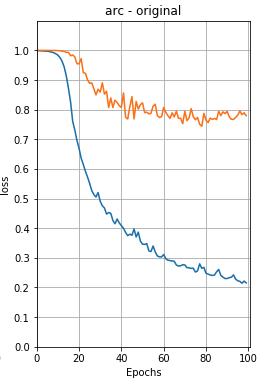
\includegraphics[width=\linewidth]{Materials/Results/Augmentation/Arc}
		\caption{Original and arc model.\newline\newline}
	\end{subfigure}
	\hfill
	\begin{subfigure}[b]{0.19\linewidth}
		\centering
		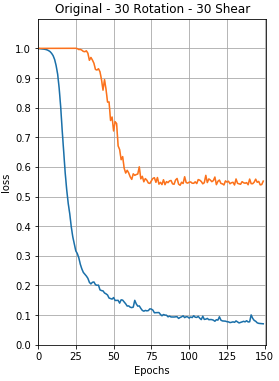
\includegraphics[width=\linewidth]{Materials/Results/Augmentation/O30R30S}
		\caption{Original, small rotations and small shearing model.\newline}
	\end{subfigure}
	\hfill
	\begin{subfigure}[b]{0.19\linewidth}
		\centering
		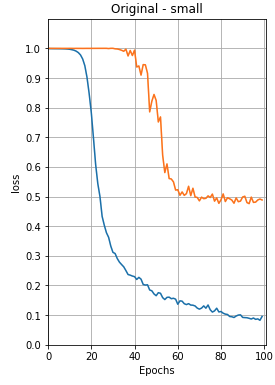
\includegraphics[width=\linewidth]{Materials/Results/Augmentation/Original}
		\caption{Original model.\newline\newline\newline}
	\end{subfigure}
	\caption{Results of training the modified U-Net model initialized with the ImageNet weights on different augmented datasets. The blue graphs indicates training loss measured with DICE, and the orange graphs indicates validation loss also measured with DICE.}
	\label{augres}
\end{figure}

\subsection{Augmentation results}
In \autoref{augres} are the results of training the modified U-Net model initialized with the ImageNet weights on different augmented training sets. We note the model achieving the lowest validation loss is the model trained on the original training set, achieving an average DICE around 0.5. The model trained on augmented data which achieves the lowest validation loss is the model trained on the original, the small rotations and the small shearing data sets, achieving an average DICE around 0.46. Although this model has been trained on 150 epochs it seems to give the same results after 100 epochs. The model trained on the original and horizontal data along with the model trained on the original and large shearing data also seems to come close to an average DICE of 0.45. Examples of prediction results can be seen in the appendix.\\
An experiment was conducted to see if it would make a difference in model performance to concatenate the datasets together rather than the fixed 506 images. In \autoref{concat} we see two models trained on the horizontal, small rotation and small shearing data sets, but one have been trained on 506 images whereas the other have had the three datasets concatenated and then shuffled. The most significant change is how fast the validation loss converges in the model trained on the concatenated dataset, although the validation loss ends being the same. We also note the training loss ends a lot higher in model trained on the concatenated data sets.

\begin{figure}
	\centering
	\begin{subfigure}[b]{0.35\linewidth}
		\centering
		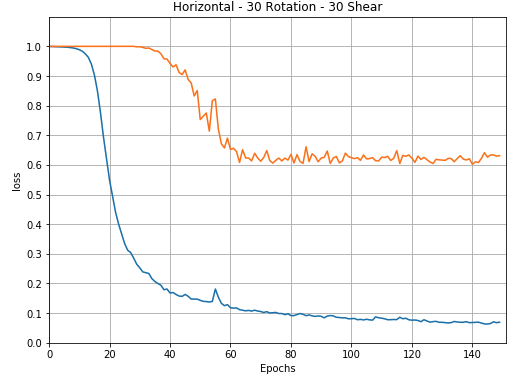
\includegraphics[width=\linewidth]{Materials/Results/Augmentation/H30R30S}
		\caption{Modified U-Net model trained on the horizontal, small rotations and small shearing datasets.\newline}
	\end{subfigure}
	\qquad
	\begin{subfigure}[b]{0.35\linewidth}
		\centering
		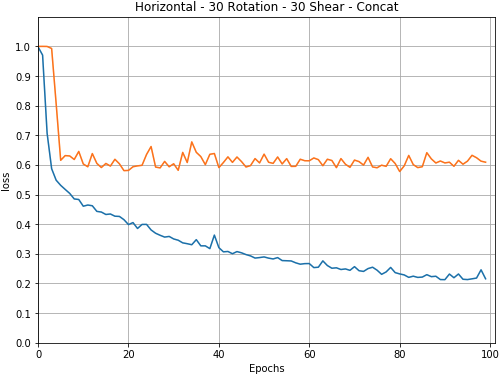
\includegraphics[width=\linewidth]{Materials/Results/Augmentation/H30R30SC}
		\caption{Modified U-Net model trained on the horizontal, small rotations and small shearing datasets concatenated and shuffled.}
	\end{subfigure}
	\caption{Experiment showing concatenating the data sets rather than picking 506 images to train on yields same validation results.}
	\label{concat}
\end{figure}

\subsection{Test results}
\begin{wraptable}{l}{0.6\linewidth}
	\centering
	\resizebox{0.55\columnwidth}{!}{%
	\begin{tabular}{|c|c|c|c|c|c|c|c|}
		\hline
		\multicolumn{2}{|c|}{ } & $t_1$ & $t_2$ & $t_3$ & $t_4$ & $t_5$ & $t_6$ \\
		\hline
		\multirow{6}{*}{Fives data}
		&\cellcolor{light-gray}Zero augmented &\cellcolor{light-gray} 0.0 &\cellcolor{light-gray} 0.0 &\cellcolor{light-gray}   0.055 &\cellcolor{light-gray} 0.038 &\cellcolor{light-gray} 0.138 &\cellcolor{light-gray} \\ \hhline{~|-|-|-|-|-|-|-|}
		&\cellcolor{light-gray}Non-zero augmented &\cellcolor{light-gray} 0.0 &\cellcolor{light-gray} 0.0 &\cellcolor{light-gray}   0.387 &\cellcolor{light-gray} 0.132 &\cellcolor{light-gray} 0.240 &\cellcolor{light-gray} \\\hhline{~|-|-|-|-|-|-|-|}
		&\cellcolor{light-gray} Relative change & \cellcolor{light-gray} 0.0 &\cellcolor{light-gray} 0.0 &\cellcolor{light-gray} 0.332 &\cellcolor{light-gray} 0.094 &\cellcolor{light-gray} 0.102 &\cellcolor{light-gray} \\\cline{2-8}
		&Zero original			   & 0.0 & 0.0 &   0.105 & 0.082 & 0.123 & \\\cline{2-8}
		&Non-zero original	    & 0.0 & 0.0 &   0.366 & 0.191 & 0.216 & \\\cline{2-8}
		& Relative change &  0.0 & 0.0 & 0.261 & 0.109 & 0.093 & \\\hline
		\multirow{6}{*}{Sixes data}
		&\cellcolor{light-gray}Zero augmented 		  &\cellcolor{light-gray} 0.0  &\cellcolor{light-gray} 0.0 \cellcolor{light-gray}&\cellcolor{light-gray}   0.067 &\cellcolor{light-gray} 0.217 &\cellcolor{light-gray} 0.318 &\cellcolor{light-gray} 0.427 \\\hhline{~|-|-|-|-|-|-|-|}
		&\cellcolor{light-gray}Non-zero augmented &\cellcolor{light-gray} 0.0 &\cellcolor{light-gray} 0.0	 &\cellcolor{light-gray} 0.667 &\cellcolor{light-gray} 0.309 &\cellcolor{light-gray} 0.398 &\cellcolor{light-gray} 0.427 \\\hhline{~|-|-|-|-|-|-|-|}
		& \cellcolor{light-gray}Relative change &\cellcolor{light-gray} 0.0 &\cellcolor{light-gray} 0.0 &\cellcolor{light-gray} 0.600 &\cellcolor{light-gray} 0.092 &\cellcolor{light-gray} 0.080 &\cellcolor{light-gray} 0.0 \\\cline{2-8}
		&Zero original			   & 0.0 & 0.059& 0.147 & 0.239 & 0.289 & 0.439 \\\cline{2-8}
		&Non-zero original	    & 0.0 & 0.198& 0.367 & 0.299 & 0.362 & 0.439 \\\cline{2-8}
		&Relative change & 0.0 & 0.139 & 0.220 & 0.060 & 0.073 & 0.0 \\\hline
	\end{tabular}%
	}
	\caption{Average DICE of each 'time interval' of the five series and six series test data.}
	\label{tableDice}
\end{wraptable}

In \autoref{onesfivessixes} the test set has been split into three separate volumes. Each of the results have been reported with and without having zero results in the average. The model trained on augmented data seems to score slightly higher or the same averages on all volumes when we do not count in zero results whereas when we do count zero results the model trained on the original training set seems to score higher. The overall results seem to be quite similar. Test results for the rest of the models can be seen in the appendix. In \autoref{tableDice} the volumes have further been split into 'time intervals'. Here we see when removing zero results the relative increase in DICE is greatest for the model trained on augmented data, and the relative increase diminishes as we move 'up in time'. In \autoref{circlecount} the performance have been measured with the circle count metric. We note for both models the regression line is quite close to have slope 1. We also note for the model trained on the original training set, that in images where the true mask count is low the predicted number of circles is high, whereas when the true mask count is high, the predicted number of circles is close to be the true number of circles. For the model trained on the augmented data we see the opposite trend.

\begin{figure}
	\centering
	\begin{subfigure}[b]{\linewidth}
		\centering
		\includegraphics[width=\linewidth]{Materials/Results/Test/Originaltest}
		\caption{Results for the model trained on the original training set.}
	\end{subfigure}
	\\
	\begin{subfigure}[b]{\linewidth}
		\centering
		\includegraphics[width=\linewidth]{Materials/Results/Test/Augtest}
		\caption{Results for the model trained on the original, small rotations and small shearing data sets.}
	\end{subfigure}
	\caption{Average DICE on test set split into three separate volumes consisting of the single series images, five series images and six series images.}
	\label{onesfivessixes}
\end{figure}

%\begin{table}
%	\centering
%	\resizebox{0.65\columnwidth}{!}{%
%	\begin{tabular}{|c|c|c|c|c|c|c|c|}
%		\hline
%		\multicolumn{2}{|c|}{ } & $t_1$ & $t_2$ & $t_3$ & $t_4$ & $t_5$ & $t_6$ \\
%		\hline
%		\multirow{6}{*}{Fives data}
%			&\cellcolor{light-gray}Zero augmented &\cellcolor{light-gray} 0.0 &\cellcolor{light-gray} 0.0 &\cellcolor{light-gray}   0.055 &\cellcolor{light-gray} 0.038 &\cellcolor{light-gray} 0.138 &\cellcolor{light-gray} \\ \hhline{~|-|-|-|-|-|-|-|}
%			&\cellcolor{light-gray}Non-zero augmented &\cellcolor{light-gray} 0.0 &\cellcolor{light-gray} 0.0 &\cellcolor{light-gray}   0.387 &\cellcolor{light-gray} 0.132 &\cellcolor{light-gray} 0.240 &\cellcolor{light-gray} \\\hhline{~|-|-|-|-|-|-|-|}
%			&\cellcolor{light-gray} Relative change & \cellcolor{light-gray} 0.0 &\cellcolor{light-gray} 0.0 &\cellcolor{light-gray} 0.332 &\cellcolor{light-gray} 0.094 &\cellcolor{light-gray} 0.102 &\cellcolor{light-gray} \\\cline{2-8}
%			&Zero original			   & 0.0 & 0.0 &   0.105 & 0.082 & 0.123 & \\\cline{2-8}
%			&Non-zero original	    & 0.0 & 0.0 &   0.366 & 0.191 & 0.216 & \\\cline{2-8}
%			& Relative change &  0.0 & 0.0 & 0.261 & 0.109 & 0.093 & \\\hline
%		\multirow{6}{*}{Sixes data}
%			&\cellcolor{light-gray}Zero augmented 		  &\cellcolor{light-gray} 0.0  &\cellcolor{light-gray} 0.0 \cellcolor{light-gray}&\cellcolor{light-gray}   0.067 &\cellcolor{light-gray} 0.217 &\cellcolor{light-gray} 0.318 &\cellcolor{light-gray} 0.427 \\\hhline{~|-|-|-|-|-|-|-|}
%			&\cellcolor{light-gray}Non-zero augmented &\cellcolor{light-gray} 0.0 &\cellcolor{light-gray} 0.0	 &\cellcolor{light-gray} 0.667 &\cellcolor{light-gray} 0.309 &\cellcolor{light-gray} 0.398 &\cellcolor{light-gray} 0.427 \\\hhline{~|-|-|-|-|-|-|-|}
%			& \cellcolor{light-gray}Relative change &\cellcolor{light-gray} 0.0 &\cellcolor{light-gray} 0.0 &\cellcolor{light-gray} 0.600 &\cellcolor{light-gray} 0.092 &\cellcolor{light-gray} 0.080 &\cellcolor{light-gray} 0.0 \\\cline{2-8}
%			&Zero original			   & 0.0 & 0.059& 0.147 & 0.239 & 0.289 & 0.439 \\\cline{2-8}
%			&Non-zero original	    & 0.0 & 0.198& 0.367 & 0.299 & 0.362 & 0.439 \\\cline{2-8}
%			&Relative change & 0.0 & 0.139 & 0.220 & 0.060 & 0.073 & 0.0 \\\hline
%	\end{tabular}%
%	}
%	\caption{Average DICE of each 'time interval' of the five series and six series test data.}
%	\label{tableDice}
%\end{table}